\documentclass[aspectratio=169,10pt]{beamer}

\usepackage[T1]{fontenc}
\usepackage{lmodern}
\usepackage{graphicx}
\usepackage{booktabs}
\usepackage{tabularx}
\usepackage{tikz}
\usepackage{amsmath}
\usepackage{ragged2e}
\usepackage{fontawesome5}

\definecolor{Ink}{HTML}{172033}
\definecolor{Muted}{HTML}{667085}
\definecolor{CanvaCyan}{HTML}{00C4CC}
\definecolor{CanvaPurple}{HTML}{7D2AE8}
\definecolor{SoftCyan}{HTML}{E7FAFA}
\definecolor{SoftPurple}{HTML}{F2EAFE}
\definecolor{Warm}{HTML}{FFB84D}

\setbeamertemplate{navigation symbols}{}
\pdfstringdefDisableCommands{\def\translate#1{#1}}
\setbeamertemplate{caption}{\raggedright\insertcaption\par}
\setbeamercolor{background canvas}{bg=white}
\setbeamercolor{normal text}{fg=Ink,bg=white}
\setbeamercolor{frametitle}{fg=Ink,bg=white}
\setbeamerfont{frametitle}{series=\bfseries,size=\Large}
\setbeamerfont{title}{series=\bfseries,size=\Huge}
\setbeamerfont{subtitle}{size=\large}
\setbeamerfont{normal text}{size=\normalsize}
\setbeamerfont{footline}{size=\scriptsize}
\setbeamercolor{itemize item}{fg=CanvaPurple}
\setbeamercolor{itemize subitem}{fg=CanvaCyan}
\setbeamercolor{block title}{fg=white,bg=CanvaPurple}
\setbeamercolor{block body}{fg=Ink,bg=SoftPurple}

\setbeamertemplate{footline}{%
  \leavevmode%
  \hbox{%
  \begin{beamercolorbox}[wd=.72\paperwidth,ht=2.8ex,dp=1.4ex,leftskip=1.1em]{footline}%
    \color{Muted}OmniStyle
  \end{beamercolorbox}%
  \begin{beamercolorbox}[wd=.28\paperwidth,ht=2.8ex,dp=1.4ex,rightskip=1.1em plus1fil]{footline}%
    \hfill\color{Muted}\insertframenumber/\inserttotalframenumber
  \end{beamercolorbox}}%
}

\newcommand{\kicker}[1]{\vspace{0.2em}{\color{CanvaPurple}\small\bfseries #1}\vspace{0.3em}}
\newcommand{\takeaway}[1]{\vspace{0.25em}{\color{Ink}\large\bfseries #1}\vspace{0.45em}}
\newcommand{\smallmuted}[1]{{\color{Muted}\small #1}}
\newcommand{\metric}[3]{%
  \begin{minipage}[t]{0.31\linewidth}
    {\color{CanvaPurple}\Large\bfseries #1}\\[-0.2em]
    {\bfseries #2}\\[-0.1em]
    {\color{Muted}\small #3}
  \end{minipage}
}
\newcommand{\iconrow}[4]{%
  \par\vspace{0.68em}\noindent%
  \begin{minipage}[t]{0.09\linewidth}
    \tikz[baseline=-0.65ex]\node[circle,draw=#1,fill=#1!10,text=#1,inner sep=2.4pt] {\scriptsize #2};
  \end{minipage}%
  \hspace{0.35em}%
  \begin{minipage}[t]{0.84\linewidth}
    {\bfseries #3}\\[-0.1em]
    {\color{Muted}\small #4}
  \end{minipage}\par%
}
\newcommand{\signalwide}[5]{%
  \begin{minipage}[t]{0.47\linewidth}
    \begin{minipage}[t]{0.11\linewidth}
      {\color{#1}\large #2}
    \end{minipage}%
    \hspace{0.25em}%
    \begin{minipage}[t]{0.82\linewidth}
      {\bfseries #3}\\[0.18em]
      {\small #4}\\[0.12em]
      {\color{Muted}\scriptsize #5}
    \end{minipage}
  \end{minipage}%
}
\newcommand{\confbadge}[2]{%
  \begin{tikzpicture}[baseline=(label.base)]
    \node[draw=#1,fill=#1!8,text=#1,line width=0.7pt,rounded corners=1.6pt,inner xsep=5pt,inner ysep=2.4pt] (label)
      {\scriptsize\bfseries #2};
  \end{tikzpicture}%
}
\newcommand{\companymark}[2]{%
  \begin{minipage}[t]{0.16\linewidth}
    \centering
    \includegraphics[width=1.34cm,height=0.70cm,keepaspectratio]{#1}\\[-0.08em]
    {\color{Muted}\scriptsize #2}
  \end{minipage}%
}
\newcommand{\researchthumb}[2]{%
  \begin{minipage}[t]{0.32\linewidth}
    \centering
    \includegraphics[width=\linewidth,height=0.205\paperheight,keepaspectratio]{#1}\\[-0.05em]
    {\color{Ink}\scriptsize\bfseries #2}
  \end{minipage}%
}
\title{OmniStyle}
\subtitle{Filtering High-Quality Style Transfer Data at Scale}
\author{Ye Wang}
\date{Research Scientist Interview}

\begin{document}

% {
% \setbeamertemplate{footline}{}
% \begin{frame}[plain]
%   \begin{tikzpicture}[remember picture,overlay]
%     \fill[CanvaCyan] (current page.south west) rectangle ([xshift=0.17\paperwidth]current page.north west);
%     \fill[CanvaPurple] ([xshift=0.17\paperwidth]current page.south west) rectangle ([xshift=0.22\paperwidth]current page.north west);
%     \node[anchor=south east,opacity=0.95] at ([xshift=-0.55cm,yshift=0.68cm]current page.south east)
%       {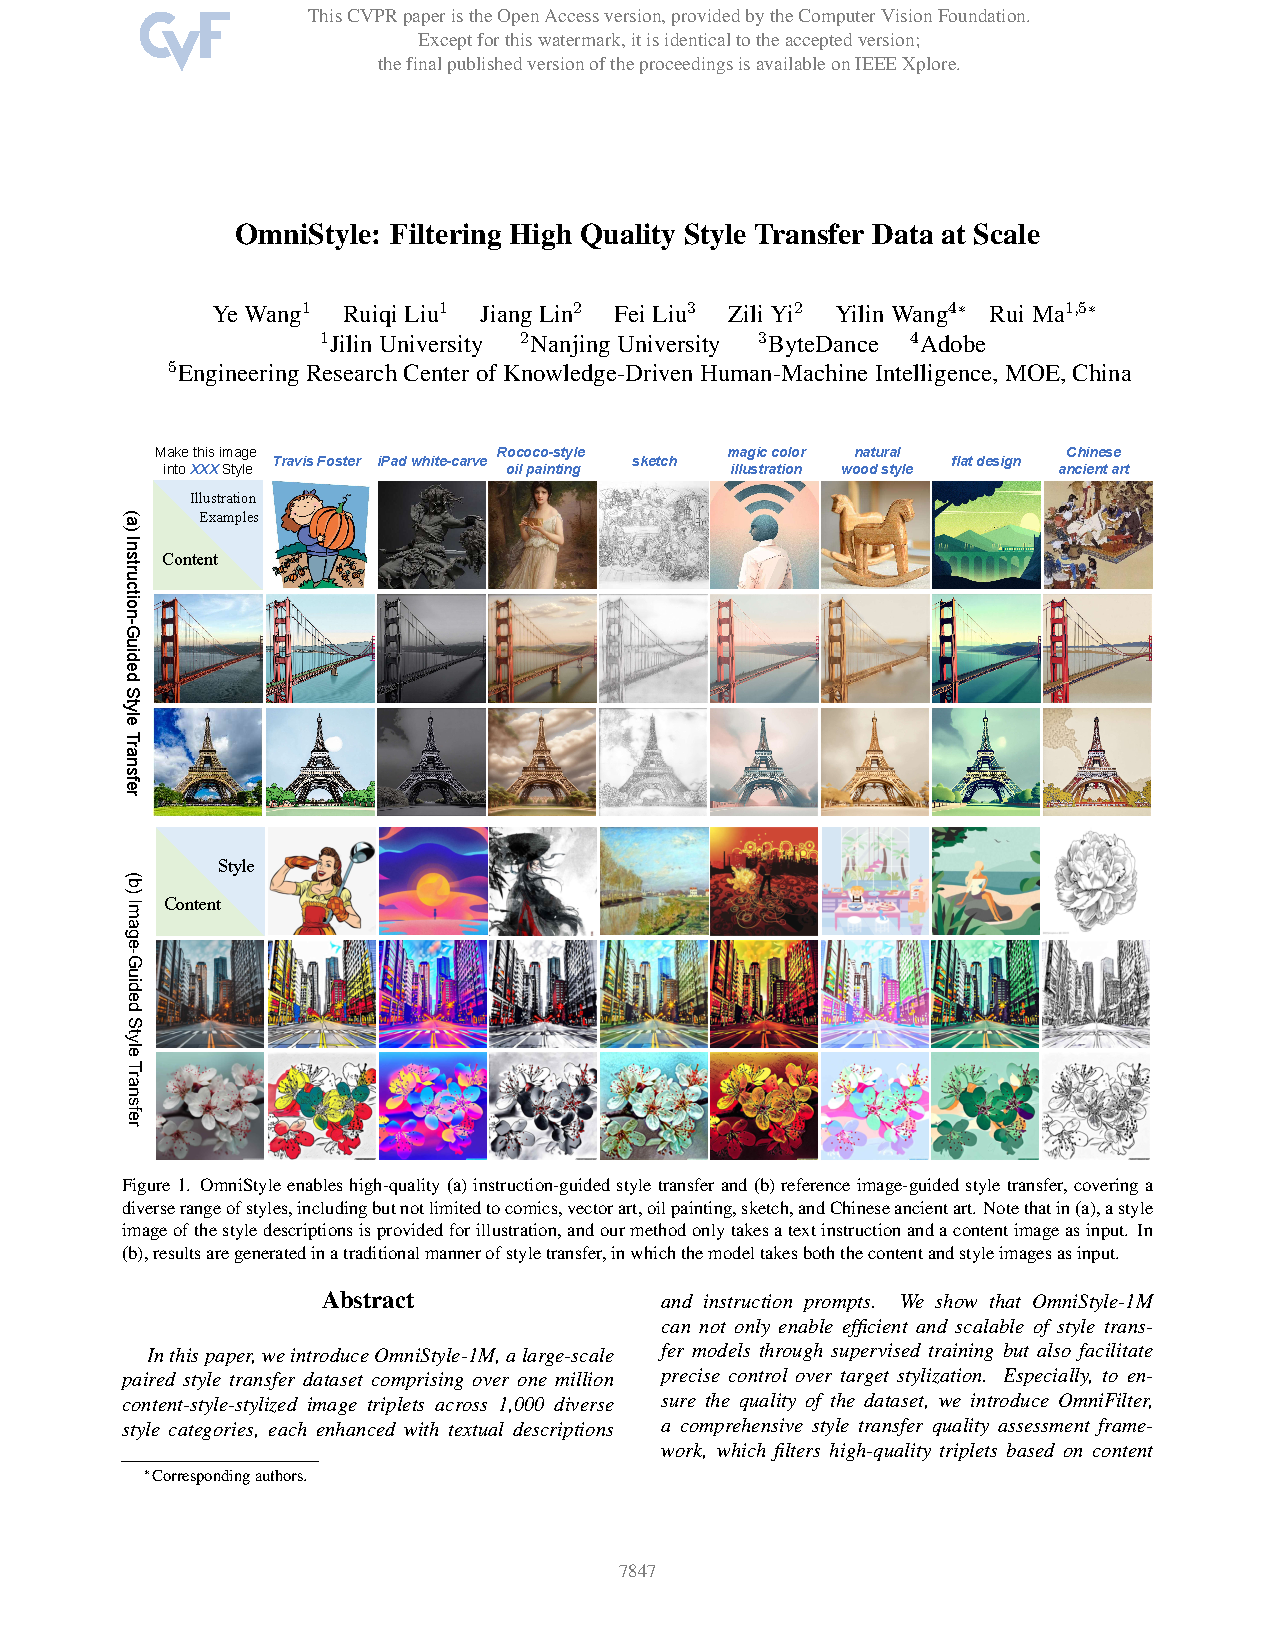
\includegraphics[page=1,width=0.34\paperwidth,trim=34 385 24 205,clip]{OmniStyle_CVPR2025_paper.pdf}};
%   \end{tikzpicture}
%   \vspace{0.82cm}
%   \hspace{0.27\paperwidth}
%   \begin{minipage}{0.37\paperwidth}
%     {\color{CanvaPurple}\small\bfseries CVPR 2025}\\[1.0em]
%     {\color{Ink}\fontsize{34}{38}\selectfont\bfseries OmniStyle}\\[0.25em]
%     {\color{Ink}\Large Filtering High-Quality\\Style Transfer Data\\at Scale}\\[1.0em]
%     {\color{Muted}\normalsize Ye Wang}
%   \end{minipage}
% \end{frame}
% }

\begin{frame}{About Me}
  
  % \takeaway{The magic you are looking for is in the work you are avoiding.}

  \begin{columns}[T,onlytextwidth]
    \column{0.56\linewidth}
    {\LARGE\bfseries Ye Wang}\\[-0.1em]
    % {\color{Muted}\small Research Scientist candidate}

    \iconrow{CanvaPurple}{\faGraduationCap}{Ph.D. candidate in AI}{Jilin University, China, expected Dec. 2026}
    \iconrow{CanvaCyan}{\faBrain}{Research direction}{Style Transfer, Image Editing, Computer Vision}

    \column{0.30\linewidth}
    \vspace{-0.15em}
    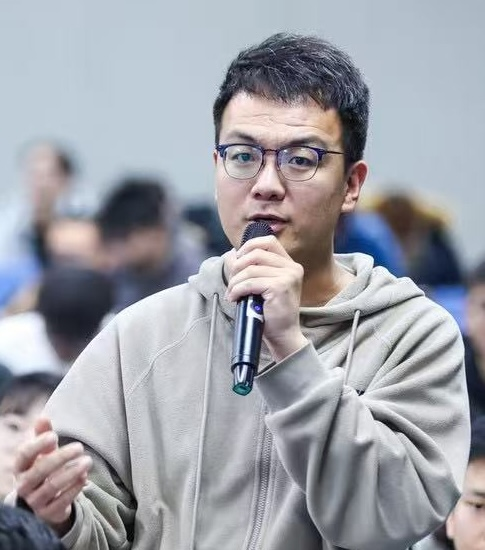
\includegraphics[width=\linewidth,trim=8 0 8 0,clip]{assets/ye_wang_profile.jpeg}
  \end{columns}
\end{frame}

\begin{frame}{About Me}
  % \kicker{TWO SIGNALS}
  \takeaway{I bring 7 publications, including 2 top-tier conference papers, plus hands-on industry research experience.}

  \vspace{0.5em}
  \begin{columns}[T,onlytextwidth]
    \column{0.10\linewidth}
      {\color{CanvaPurple}\Large\faIcon{file-alt}}
    \column{0.86\linewidth}
      {\bfseries Research output}\\[-0.05em]
      {\color{Muted}\small 7 papers in total, including 2 top-tier conference papers}\\[0.55em]
      \confbadge{CanvaPurple}{CVPR 2025}\hspace{0.45em}
      \confbadge{CanvaCyan}{AAAI 2025}\hspace{0.45em}
      \confbadge{Warm}{ECCV Submit}\hspace{0.45em}
      \confbadge{CanvaPurple}{NeurIPS Submit}
  \end{columns}

  \vspace{0.75em}
  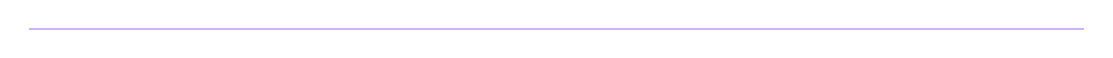
\begin{tikzpicture}
    \draw[CanvaPurple!35,line width=0.7pt] (0,0) -- (13.4,0);
  \end{tikzpicture}

  \vspace{0.6em}
  \begin{columns}[T,onlytextwidth]
    \column{0.10\linewidth}
      {\color{CanvaCyan}\Large\faBriefcase}
    \column{0.86\linewidth}
      {\bfseries Industry research experience}\\[-0.05em]
      {\color{Muted}\small \textbf{\color{Warm}Tencent Qingyun Talent Program}, plus research internships at Alibaba, Baidu, JD.com, and Kunlun Tech}\\[0.42em]
      \companymark{assets/logos/tencent.png}{\shortstack{Tencent\\Qingyun}}
      \hfill
      \companymark{assets/logos/alibaba.png}{Alibaba}
      \hfill
      \companymark{assets/logos/baidu.png}{Baidu}
      \hfill
      \companymark{assets/logos/jingdong.jpeg}{JD.com}
      \hfill
      \companymark{assets/logos/kunlun.png}{Kunlun}
  \end{columns}

  \vspace{0.82em}
  {\color{Muted}\scriptsize Note: {\color{Warm}\textbf{Tencent Qingyun Talent Program}} is Tencent's highly selective track for outstanding student researchers and engineers.}
\end{frame}

\begin{frame}{Research Overview}
  \vspace{0.1em}
  \centering
  \researchthumb{assets/sigstyle.png}{SigStyle}
  \hfill
  \researchthumb{assets/omnistyle.png}{OmniStyle}
  \hfill
  \researchthumb{assets/omnistyle2.png}{OmniStyle2}

  \vspace{0.55em}

  \researchthumb{assets/SVG.png}{SVG}
  \hfill
  \researchthumb{assets/font.png}{Font}
  \hfill
  \researchthumb{assets/umm-posttraining.png}{UMM}
\end{frame}

\begin{frame}[plain]
  \begin{tikzpicture}[remember picture,overlay]
    \fill[CanvaPurple!5] (current page.south west) rectangle (current page.north east);
    \fill[CanvaPurple] (current page.south west) rectangle ([xshift=0.17\paperwidth]current page.north west);
    \fill[CanvaCyan] ([xshift=0.17\paperwidth]current page.south west) rectangle ([xshift=0.21\paperwidth]current page.north west);
    % \node[anchor=south east,opacity=0.96] at ([xshift=-0.55cm,yshift=0.62cm]current page.south east)
    %   {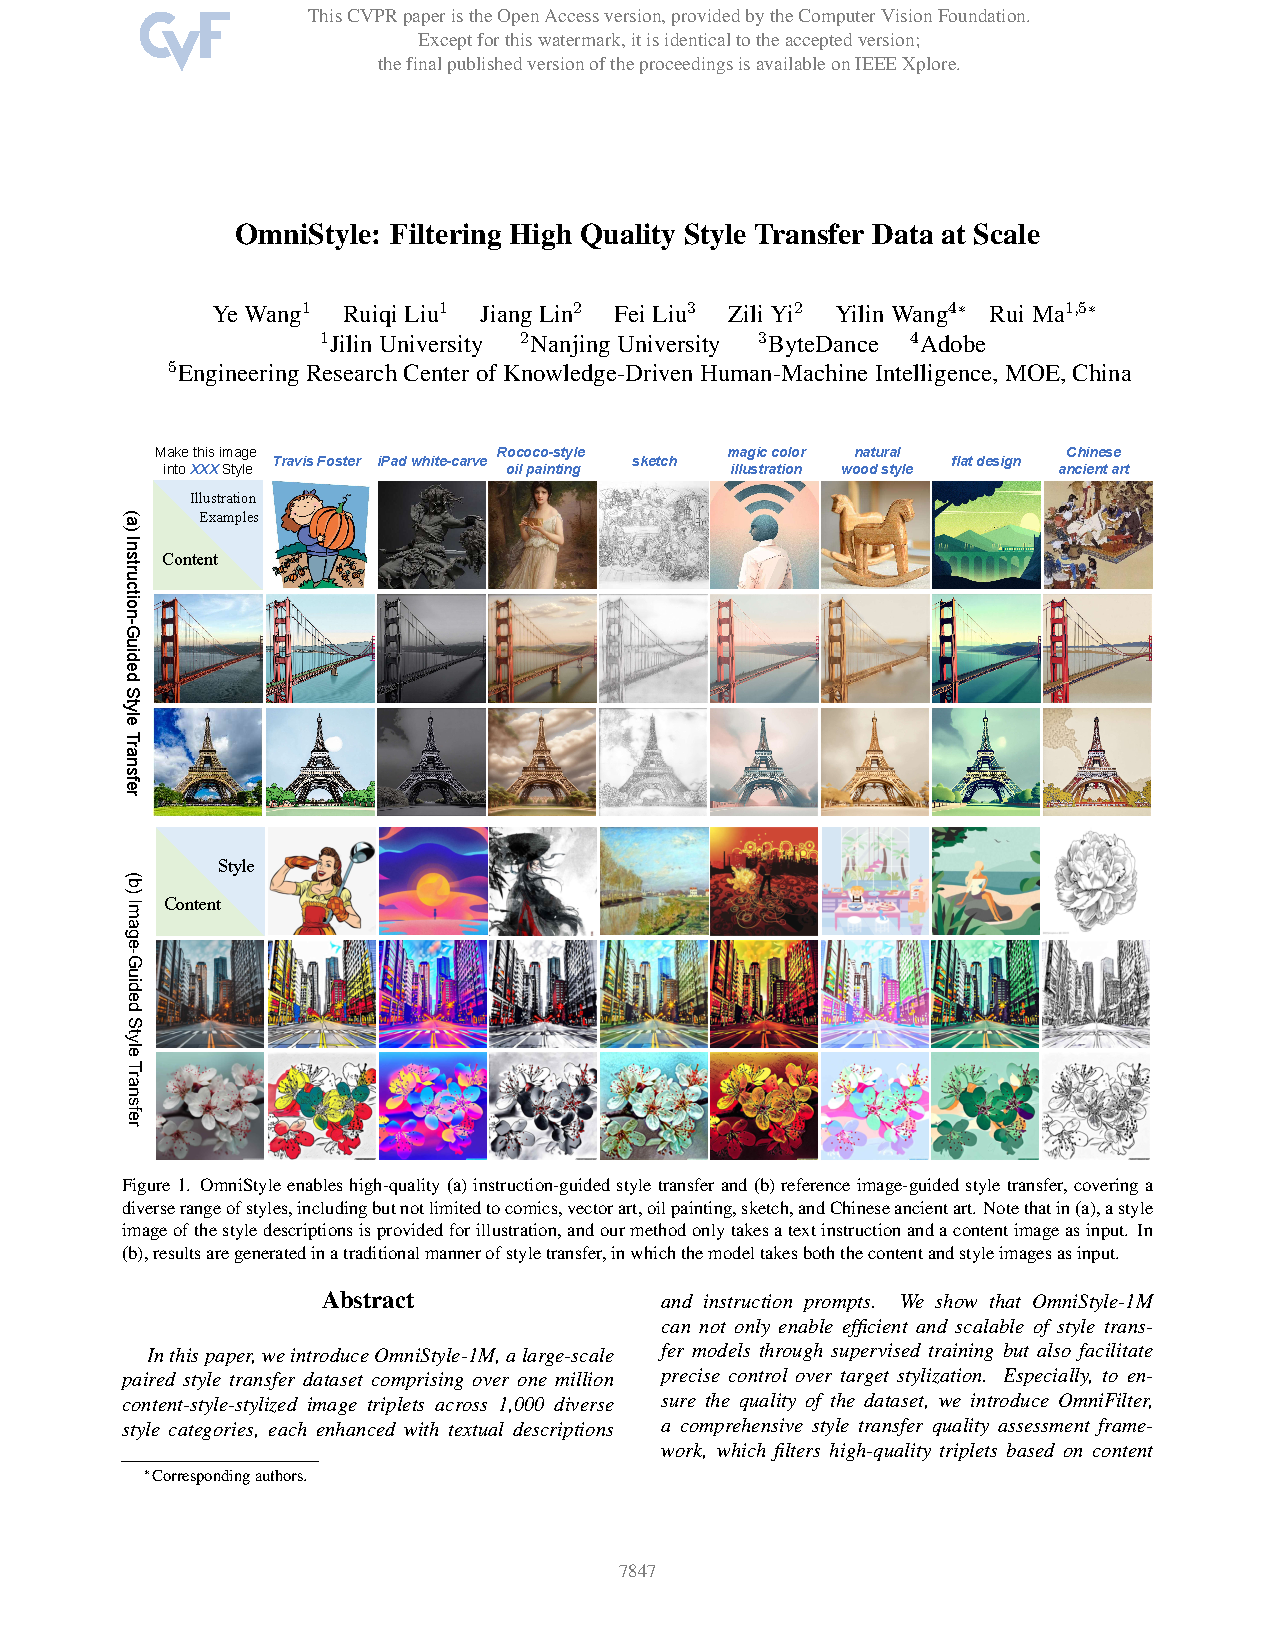
\includegraphics[page=1,width=0.34\paperwidth,trim=34 385 24 205,clip]{OmniStyle_CVPR2025_paper.pdf}};
  \end{tikzpicture}

  \vspace{0.9cm}
  \hspace{0.26\paperwidth}
  \begin{minipage}{0.60\paperwidth}
    {\color{CanvaPurple}\small\bfseries CVPR 2025}\\[1.0em]
    {\color{Ink}\fontsize{32}{36}\selectfont\bfseries OmniStyle}\\[0.3em]
    {\color{Ink}\Large Filtering High-Quality Style Transfer Data at Scale}
    % {\color{Muted}\normalsize What was the problem, and how did we solve it?}
  \end{minipage}
\end{frame}

\begin{frame}{Motivation}
  \kicker{WHY THIS PROBLEM MATTERS}
  \takeaway{The paper starts from three limits in previous style transfer methods.}

  \begin{columns}[T,onlytextwidth]
    \column{0.32\linewidth}
    {\color{CanvaPurple}\Large\bfseries 01}\\
    {\bfseries Limited generalization}\\
    \smallmuted{Hard to handle truly arbitrary, fine-grained styles.}

    \column{0.32\linewidth}
    {\color{CanvaCyan}\Large\bfseries 02}\\
    {\bfseries Weak controllability}\\
    \smallmuted{Unsupervised stylization can introduce artifacts or distortion.}

    \column{0.32\linewidth}
    {\color{Warm}\Large\bfseries 03}\\
    {\bfseries Low efficiency}\\
    \smallmuted{Optimization or inversion makes deployment expensive.}
  \end{columns}

  \vspace{1.0em}
  {\color{CanvaPurple}\bfseries Key question:}
  {\color{Muted} can we build a controllable and efficient end-to-end style transfer system by learning from better paired data?}
\end{frame}

\begin{frame}{Our Solution}
  \kicker{DATA-CENTRIC PIPELINE}
  \takeaway{Our answer was to turn style transfer into a supervised learning pipeline built on filtered paired data.}

  \centering
  \begin{minipage}[t]{0.27\linewidth}
    \raggedright
    {\color{CanvaPurple}\Large\bfseries 01}\\
    {\bfseries Construct data}\\
    \smallmuted{Build \textbf{OmniStyle-1M}, a paired dataset for stylization learning.}
  \end{minipage}%
  \begin{minipage}[t]{0.06\linewidth}
    \centering
    \vspace{1.7em}
    {\color{Muted}\Large\faLongArrowAltRight}
  \end{minipage}%
  \begin{minipage}[t]{0.27\linewidth}
    \raggedright
    {\color{CanvaCyan}\Large\bfseries 02}\\
    {\bfseries Filter data quality}\\
    \smallmuted{Use \textbf{OmniFilter} to keep the best triplets with task-specific signals.}
  \end{minipage}%
  \begin{minipage}[t]{0.06\linewidth}
    \centering
    \vspace{1.7em}
    {\color{Muted}\Large\faLongArrowAltRight}
  \end{minipage}%
  \begin{minipage}[t]{0.27\linewidth}
    \raggedright
    {\color{Warm}\Large\bfseries 03}\\
    {\bfseries Train the model}\\
    \smallmuted{Train \textbf{OmniStyle}, one feed-forward DiT for two stylization modes.}
  \end{minipage}

  \vspace{1.0em}
  {\color{CanvaPurple}\bfseries Bridge:}
  {\color{Muted} the next seven slides unpack data creation first, then OmniFilter across four views, then training.}
\end{frame}

\begin{frame}{Step 1: OmniStyle-1M Overview}
  \kicker{PIPELINE STEP 1}
  \takeaway{OmniStyle-1M is a million-scale triplet dataset with broad style coverage and diverse content.}

  \centering
  
\includegraphics[width=0.8\linewidth]{/Users/killerwang/Documents/Canva-Interview/assets/triplets.png}

  \vspace{0.55em}
  \metric{1M+}{triplets}{content, style, stylized result}
  \hfill
  \metric{1,000}{style categories}{fine-grained style coverage}
  \hfill
  \metric{20}{content categories}{broad content diversity}
\end{frame}

\begin{frame}{Step 1: How We Built OmniStyle-1M}
  \kicker{PIPELINE STEP 1}
  \takeaway{We generate content images, pair them with style references, and create multiple stylized candidates per pair.}

  \small
  \begin{itemize}
    \item Generate content images with FLUX across 20 content categories.
    \item Collect style reference images from Style30K across 1,000 style categories.
    \item Form content-style pairs and run six existing style transfer models.
    \item Keep all candidates at this stage; filtering happens in the next step.
  \end{itemize}

  \vspace{0.2em}
  {\color{Warm}\bfseries Pipeline example}\\[-0.1em]
  {\color{Muted}\small The full pairing and candidate-generation workflow is illustrated below.}

  \vspace{0.5em}
  \centering
  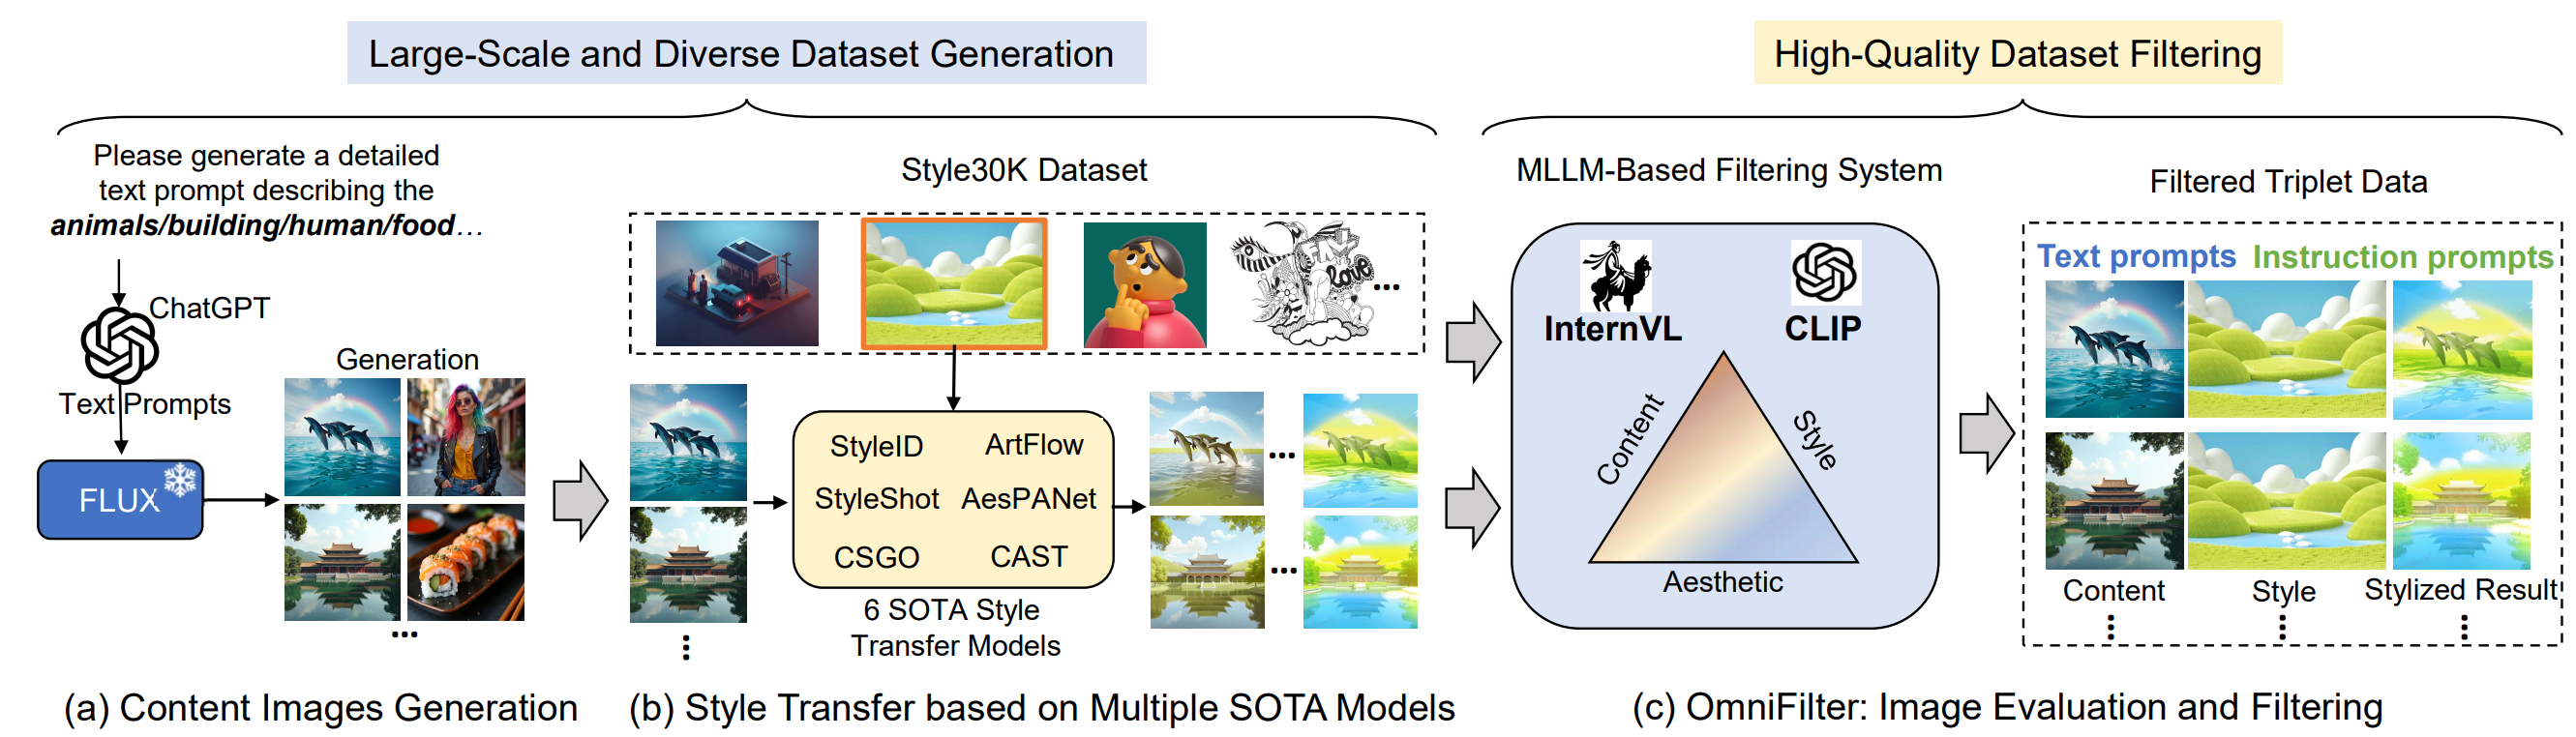
\includegraphics[width=\linewidth,height=0.34\textheight,keepaspectratio]{assets/build_dataset.png}
\end{frame}

\begin{frame}{Step 2: OmniFilter Overview}
  \kicker{PIPELINE STEP 2}
  \takeaway{OmniFilter is the filtering step that turns multiple raw stylizations into one training example.}

  \begin{columns}[T,onlytextwidth]
    \column{0.48\linewidth}
    \small
    \begin{itemize}
      \item \textbf{Input}: 1 content image, 1 style reference, and 6 generated stylizations.
      \item \textbf{Process}: score each candidate with three dimension checks.
      \item \textbf{Output}: keep the best candidate and discard the other five.
    \end{itemize}

    \vspace{0.35em}
    {\color{Muted}\small This gives us a cleaner dataset for training OmniStyle.}

    \column{0.48\linewidth}
    \centering
    \resizebox{\linewidth}{!}{%
    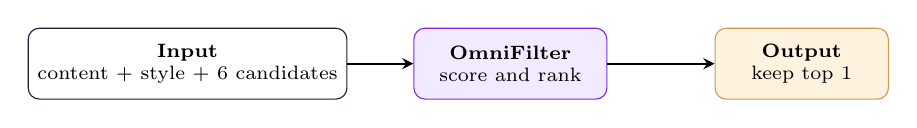
\begin{tikzpicture}[font=\scriptsize,>=stealth]
      \node[draw=Ink,rounded corners=4pt,minimum width=2.85cm,minimum height=0.9cm,fill=white,align=center] (input) at (0,0) {\bfseries Input\\content + style + 6 candidates};
      \node[draw=CanvaPurple,rounded corners=4pt,minimum width=2.45cm,minimum height=0.9cm,fill=SoftPurple,align=center] (filter) at (4.1,0) {\bfseries OmniFilter\\score and rank};
      \node[draw=Warm!80!Ink,rounded corners=4pt,minimum width=2.2cm,minimum height=0.9cm,fill=Warm!18,align=center] (output) at (7.8,0) {\bfseries Output\\keep top 1};
      \draw[->,thick] (input) -- (filter);
      \draw[->,thick] (filter) -- (output);
    \end{tikzpicture}}

    \vspace{0.7em}
    {\bfseries Three dimensions}\\[0.35em]
    {\small
    {\color{CanvaPurple}\bfseries Content}: preserve subject and layout\\[0.35em]
    {\color{CanvaCyan}\bfseries Style}: match the target reference\\[0.35em]
    {\color{Warm}\bfseries Aesthetic}: keep the result visually strong
    }
  \end{columns}
\end{frame}

\begin{frame}{Step 2A: Content Preservation}
  \kicker{PIPELINE STEP 2 / SIGNAL 1}
  \takeaway{The first signal checks whether stylization keeps the original subjects, semantics, and spatial structure.}

  \begin{columns}[T,onlytextwidth]
    \column{0.57\linewidth}
    \small
    \begin{itemize}
      \item Content preservation combines semantic consistency and structural integrity.
      \item Semantic consistency: compare the stylized image with the content caption using CLIP image-text similarity.
      \item Structural integrity: compare content and stylized image embeddings with DINOv2.
      \item The final score gives equal weight to both parts, so the output must keep both meaning and layout.
    \end{itemize}

    \vspace{0.25em}
    \small
    \begin{align*}
      C_{score} = 0.5\,S_{semantic} + 0.5\,S_{structural}
    \end{align*}

    \column{0.38\linewidth}
    {\bfseries Content score pipeline}\\[0.4em]
    \centering
    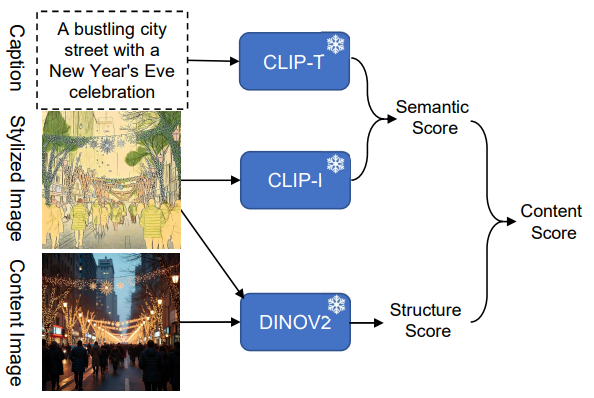
\includegraphics[width=\linewidth,height=0.58\textheight,keepaspectratio]{assets/content.png}

    \par\vspace{0.35em}
    {\color{Muted}\small CLIP measures semantic alignment, and DINOv2 measures structural preservation.}
  \end{columns}
\end{frame}

\begin{frame}{Step 2B: Style Consistency}
  \kicker{PIPELINE STEP 2 / SIGNAL 2}
  \takeaway{The second signal checks whether the output really matches the target reference style, not just a generic artistic look.}

  \begin{columns}[T,onlytextwidth]
    \column{0.57\linewidth}
    \small
    \begin{itemize}
      \item Style is subjective, so hand-crafted losses are not enough for reliable filtering.
      \item We use Style30K as supervision: same-style images are positive pairs and different-style images are negative pairs.
      \item Contrastive learning fine-tunes a CLIP image encoder so same styles cluster together in the embedding space.
      \item The similarity between the style reference and the stylized output becomes the style consistency score.
    \end{itemize}

    \vspace{0.35em}
    {\color{Muted}\small Score by embedding similarity between the target style image and the generated result.}

    \column{0.38\linewidth}
    {\bfseries Style score pipeline}\\[0.4em]
    \centering
    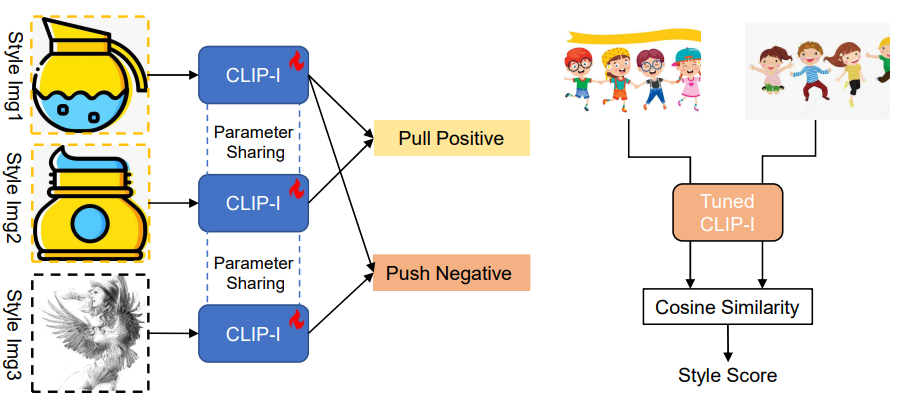
\includegraphics[width=\linewidth,height=0.58\textheight,keepaspectratio]{assets/style.png}

    \par\vspace{0.35em}
    {\color{Muted}\small Positive pairs are pulled together, negative pairs are pushed apart, and cosine similarity gives the final style score.}
  \end{columns}
\end{frame}

\begin{frame}{Step 2C: Aesthetic Appeal}
  \kicker{PIPELINE STEP 2 / SIGNAL 3}
  \takeaway{The third signal rewards outputs that are not only correct, but also visually compelling.}

  \small
  \begin{itemize}
    \setlength{\itemsep}{0.25em}
    \item Many style-transfer metrics ignore visual quality, so OmniFilter adds a dedicated aesthetic scorer.
    \item We define 40 visual attributes, including composition, balance, color harmony, lighting, contrast, and saturation.
    \item InternVL2 generates attribute captions, and we combine caption features with image features.
    \item An MLP predicts the final score, trained on AVA first and then fine-tuned on BAID to adapt to artistic images.
  \end{itemize}

  \vspace{0.25em}
  {\bfseries Attribute-based scoring}\\[0.35em]
  {\color{Muted}\small InternVL2 extracts attribute text, InternVL-G encodes both modalities, and an MLP regresses the final aesthetic score.}\\[0.55em]

  \centering
  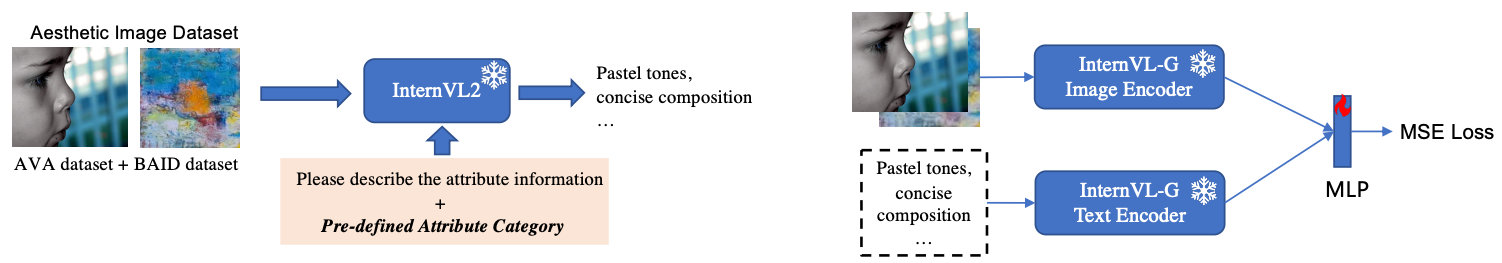
\includegraphics[width=\linewidth,height=0.34\textheight,keepaspectratio]{assets/aesthetic.png}
\end{frame}

\begin{frame}{Step 3: Train the Model (OmniStyle)}
  \kicker{PIPELINE STEP 3}
  \takeaway{A single DiT-based model handles both text-guided and image-guided stylization.}

  \begin{columns}[T,onlytextwidth]
    \column{0.65\linewidth}
    \centering
    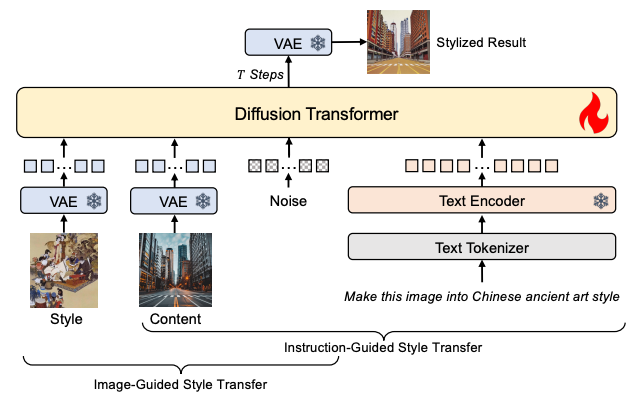
\includegraphics[width=\linewidth,height=0.52\textheight,keepaspectratio]{assets/model.png}

    \column{0.31\linewidth}
    \small
    \begin{itemize}
      \setlength{\itemsep}{0.18em}
      \item Built on FLUX-dev / MM-DiT.
      \item VAEs encode content and style inputs.
      \item Image and text tokens join noisy latents.
      \item Only the diffusion transformer is fine-tuned; the other modules stay frozen.
    \end{itemize}
  \end{columns}
\end{frame}

\begin{frame}{QUANTITATIVE EVALUATION}
  % \kicker{QUANTITATIVE EVALUATION}
  \takeaway{OmniStyle leads on style consistency while staying competitive on content preservation and aesthetic quality.}

  \begin{columns}[T,onlytextwidth]
    \column{0.49\linewidth}
    \centering
    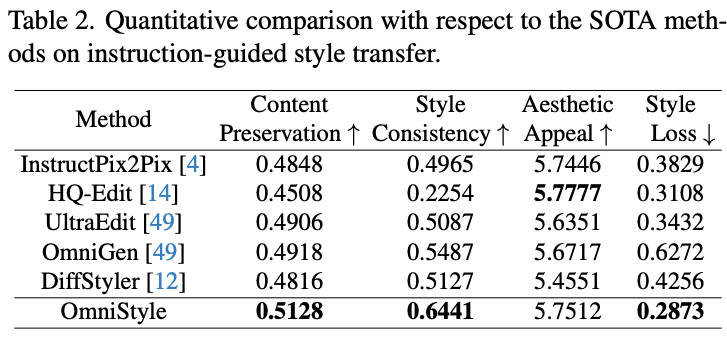
\includegraphics[width=\linewidth,height=0.54\textheight,keepaspectratio]{assets/table1.png}

    \column{0.49\linewidth}
    \centering
    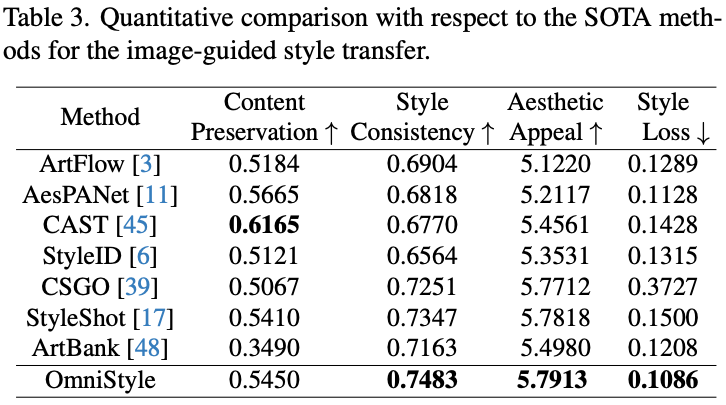
\includegraphics[width=\linewidth,height=0.54\textheight,keepaspectratio]{assets/table2.png}
  \end{columns}

  \vspace{0.4em}
  \smallmuted{Left: instruction-guided comparison. Right: image-guided comparison.}
\end{frame}

\begin{frame}{Qualitative EVALUATION}
  \kicker{INSTRUCTION-GUIDED RESULTS}
  \takeaway{The model preserves identity and layout while applying fine-grained styles in the instruction-guided setting.}

  \centering
  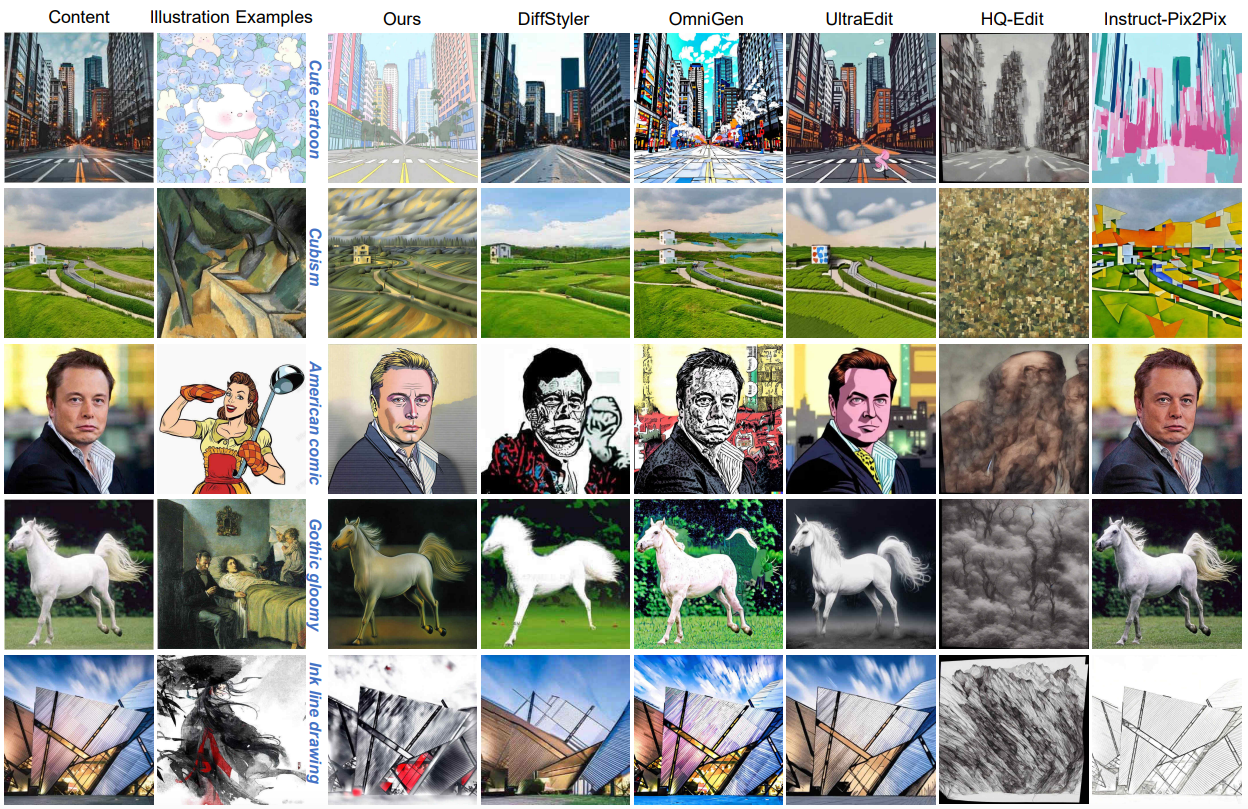
\includegraphics[width=\linewidth,height=0.58\textheight,keepaspectratio]{assets/res1.png}

  \vspace{0.25em}
  \smallmuted{Instruction-guided comparisons highlight stronger content preservation with more stable stylization across varied references.}
\end{frame}

\begin{frame}{Qualitative EVALUATION}
  \kicker{IMAGE-GUIDED RESULTS}
  \takeaway{The same model transfers color, texture, and composition reliably from a single style reference image.}

  \centering
  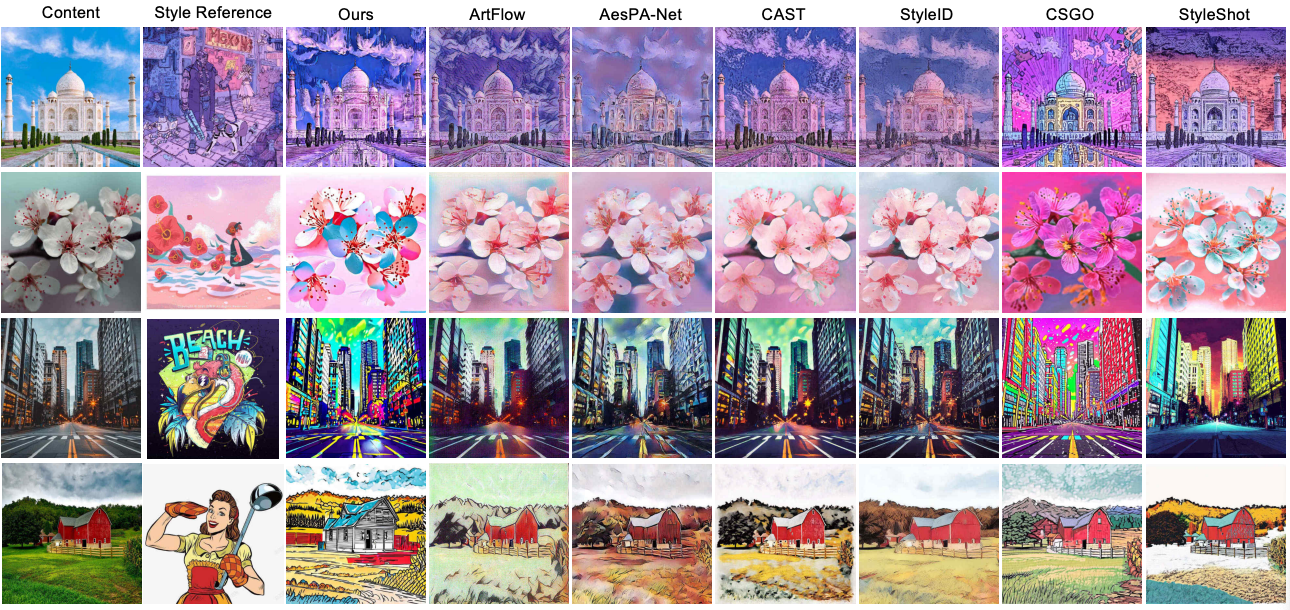
\includegraphics[width=\linewidth,height=0.58\textheight,keepaspectratio]{assets/res2.png}

  \vspace{0.25em}
  \smallmuted{Reference-image comparisons show closer style matching while keeping the original scene structure intact.}
\end{frame}

% \begin{frame}{Why This Matters for Canva}
%   \kicker{PRODUCT RELEVANCE}
%   \takeaway{The research maps naturally to controllable creative generation.}

%   \begin{columns}[T,onlytextwidth]
%     \column{0.31\linewidth}
%     {\color{CanvaPurple}\Large\bfseries Creative control}\\
%     \smallmuted{Users need predictable style transfer from either text instructions or visual references.}

%     \column{0.31\linewidth}
%     {\color{CanvaCyan}\Large\bfseries Data flywheel}\\
%     \smallmuted{High-quality filtering can turn noisy generated candidates into useful training data.}

%     \column{0.31\linewidth}
%     {\color{Warm}\Large\bfseries Production path}\\
%     \smallmuted{A feed-forward model is easier to optimize, batch, distill, and deploy than iterative pipelines.}
%   \end{columns}

%   \vspace{1.0em}
%   \begin{tikzpicture}
%     \draw[CanvaPurple,line width=2pt] (0,0) -- (13.75,0);
%     \node[anchor=west,text width=13.15cm] at (0,0.55)
%       {For a design platform, the long-term question is not just image quality. It is controllability, speed, evaluation, safety, and user trust.};
%   \end{tikzpicture}
% \end{frame}

% \begin{frame}{Closing}
%   \kicker{OMNISTYLE TAKEAWAY}
%   \takeaway{The main lesson is that better data curation can be as important as model architecture for controllable generation.}

%   \vspace{0.5em}
%   \begin{itemize}
%     \item Define quality in task terms: content preservation, style consistency, and aesthetics.
%     \item Use filtering to convert noisy synthetic candidates into useful training data.
%     \item Train a simpler feed-forward model on the filtered pairs, then evaluate with both metrics and human preference.
%   \end{itemize}

%   \vspace{0.95em}
%   {\color{Muted}Thank you. I am happy to go deeper into any stage of the pipeline.}
% \end{frame}

% \appendix

% \begin{frame}{What I Can Deep Dive Into}
%   \kicker{FOR TECHNICAL Q\&A}
%   \takeaway{I can explain the research from algorithms to engineering tradeoffs.}

%   \begin{columns}[T,onlytextwidth]
%     \column{0.49\linewidth}
%     {\bfseries Algorithmic topics}
%     \begin{itemize}
%       \item diffusion / DiT formulation
%       \item text-token and image-token conditioning
%       \item content-style disentanglement failure modes
%       \item metric design and metric limitations
%     \end{itemize}

%     \column{0.49\linewidth}
%     {\bfseries Engineering topics}
%     \begin{itemize}
%       \item large-scale data generation and filtering
%       \item distributed training and memory bottlenecks
%       \item profiling, inference speed, and distillation
%       \item evaluation loops for production quality
%     \end{itemize}
%   \end{columns}
% \end{frame}

\begin{frame}{Summary}
  \kicker{KEY TAKEAWAYS}
  \takeaway{The paper can be summarized as a data pipeline: build the dataset, filter quality, then train one unified model.}

  \vspace{0.4em}
  \begin{itemize}
    \item \textbf{Dataset:} OmniStyle-1M constructs large-scale triplets of content images, style references, and stylized results, giving the model broad supervision across diverse styles and scenes.
    \item \textbf{Filter:} OmniFilter scores candidates on content preservation, style consistency, and aesthetic appeal, then keeps the best examples for training.
    \item \textbf{Model:} OmniStyle is a unified DiT-based feed-forward model that supports both instruction-guided and image-guided stylization with strong controllability.
  \end{itemize}
\end{frame}

% \begin{frame}{Backup: Limitations and Next Steps}
%   \kicker{HONEST RESEARCH VIEW}
%   \takeaway{The next step is stronger human-aligned evaluation and faster deployment.}

%   \begin{itemize}
%     \item Synthetic data is powerful, but it can inherit biases and artifacts from source generators.
%     \item Automatic metrics help scale filtering, but human preference is still important for creative quality.
%     \item The current model can be further improved with professional artist annotations, preference learning, and distillation.
%     \item For production, I would add safety filtering, latency profiling, style-intensity controls, and online feedback loops.
%   \end{itemize}
% \end{frame}

\end{document}
